% ============================================================================
%  Argumentation Engine and Strategic Argumentation  --  Assignment 3 report
%  Build (from the report/ directory):  tectonic report.tex
% ============================================================================
% ---- course -----------------------------------------------------------------
\newcommand{\coursename}{Autonomous Systems}
% ----------------------------------------------------------------------------
\documentclass[10pt,a4paper]{article}
\usepackage[a4paper,margin=2.1cm,top=2.4cm,bottom=2.3cm,headheight=14pt]{geometry}
\usepackage{fontspec}
\usepackage{unicode-math}
% macOS fonts when installed; open look-alikes otherwise (same layout on any machine)
% (TeX Gyre fonts are loaded by file name, so the build also works with tectonic / without system fonts)
\newcommand{\gyre}[2]{#1{#2}[Extension=.otf,UprightFont=*-regular,BoldFont=*-bold,ItalicFont=*-italic,BoldItalicFont=*-bolditalic]}
\IfFontExistsTF{STIXGeneral}{\setmainfont{STIXGeneral}}{\gyre\setmainfont{texgyretermes}}
\IfFontExistsTF{STIX Two Math}{\setmathfont{STIX Two Math}}{\setmathfont{latinmodern-math.otf}}
\IfFontExistsTF{Avenir Next}{\setsansfont{Avenir Next}}{\gyre\setsansfont{texgyreheros}}
\IfFontExistsTF{Menlo}{\setmonofont{Menlo}[Scale=0.80]}{\setmonofont{DejaVuSansMono.ttf}[Scale=0.80,BoldFont=DejaVuSansMono-Bold.ttf]}
\usepackage[table]{xcolor}
\usepackage{graphicx,float,booktabs,array,tabularx,multicol,enumitem,amsmath,pifont,lastpage,ragged2e}
\usepackage[skip=4pt]{caption}
\usepackage{subcaption}
\usepackage{titlesec,fancyhdr,needspace}
\newcommand{\sectionbreak}{\needspace{9\baselineskip}}
\newcommand{\subsectionbreak}{\needspace{6\baselineskip}}
\usepackage[skins,breakable]{tcolorbox}
\usepackage{tikz}
\usetikzlibrary{positioning,shapes.geometric,calc,fit,backgrounds,arrows.meta}
\usepackage{microtype}
\usepackage[hidelinks]{hyperref}

% ---- palette (matches the figures) ----------------------------------------
\definecolor{brand}{HTML}{1B3A5C}
\definecolor{accent}{HTML}{2A78D6}
\definecolor{agx}{HTML}{1F77B4}
\definecolor{agy}{HTML}{D62728}
\definecolor{agz}{HTML}{2CA02C}
\definecolor{violetc}{HTML}{4A3AA7}
\definecolor{good}{HTML}{0E7C4A}
\definecolor{bad}{HTML}{B3261E}
\definecolor{muted}{HTML}{5F6B7A}
\definecolor{rowalt}{HTML}{F3F6FA}
\definecolor{ennbg}{HTML}{E2EDFB}
\definecolor{keybg}{HTML}{EEF5FD}
\definecolor{warnbg}{HTML}{FFF6E5}
\definecolor{warnc}{HTML}{C47F00}
\hypersetup{colorlinks=true,linkcolor=accent,urlcolor=accent,citecolor=accent}

% ---- headings ---------------------------------------------------------------
\titleformat{\section}{\sffamily\LARGE\bfseries\color{brand}}
  {\colorbox{brand}{\makebox[1.25em][c]{\color{white}\thesection}}}{0.55em}{}
  [\vspace{-2pt}{\color{accent}\titlerule[1.2pt]}]
\titleformat{\subsection}{\sffamily\Large\bfseries\color{brand}}{\color{accent}\thesubsection}{0.6em}{}
\titleformat{\subsubsection}{\sffamily\large\bfseries\color{brand}}{}{0em}{}
\titlespacing*{\section}{0pt}{16pt}{9pt}
\titlespacing*{\subsection}{0pt}{12pt}{5pt}
\titlespacing*{\subsubsection}{0pt}{9pt}{3pt}
\setcounter{secnumdepth}{2}
\setcounter{tocdepth}{2}

% ---- header / footer --------------------------------------------------------
\pagestyle{fancy}
\fancyhf{}
\renewcommand{\headrule}{{\color{accent}\hrule height 0.6pt}}
\fancyhead[L]{\sffamily\footnotesize\color{muted} Argumentation Engine and Strategic Argumentation}
\fancyhead[R]{\sffamily\footnotesize\color{muted}\nouppercase{\leftmark}}
\fancyfoot[L]{\sffamily\footnotesize\color{muted}\coursename\ -- Assignment 3 Report}
\fancyfoot[R]{\sffamily\footnotesize\color{brand}\bfseries\thepage\,{\normalfont\color{muted}/\,\pageref{LastPage}}}
\renewcommand{\sectionmark}[1]{\markboth{\thesection\quad #1}{}}

% ---- captions, lists, tables ------------------------------------------------
\captionsetup{font=small,labelfont={sf,bf,color=brand},textfont={color=black!85},labelsep=period}
\setlist{itemsep=2pt,topsep=3pt,parsep=0pt}
\setlist[itemize]{label={\color{accent}\small$\blacktriangleright$}}
\newcommand{\thd}[1]{\textcolor{white}{\sffamily\bfseries #1}}
\renewcommand{\arraystretch}{1.18}
\setlength{\tabcolsep}{5pt}
\setlength{\emergencystretch}{2.5em}
\newcommand{\yes}{\textcolor{good}{\ding{51}}}
\newcommand{\no}{\textcolor{bad}{\ding{55}}}
\newcommand{\code}[1]{\textcolor{brand!85!black}{\texttt{#1}}}
\newcommand{\kw}[1]{\textsf{\bfseries\color{brand}#1}}
\newcommand{\hl}[1]{\textbf{\color{brand}#1}}
\newcommand{\tabend}{\arrayrulecolor{brand}\specialrule{0.8pt}{0pt}{0pt}\arrayrulecolor{black}}
% argumentation notation
\newcommand{\att}{\rightharpoonup}          % attack relation  ⇀
\newcommand{\AF}{\langle\mathcal{A},\att\rangle}
\newcommand{\Args}{\mathcal{A}}
\newcommand{\GE}{\mathit{GE}}
\newcommand{\idef}{\hookrightarrow}         % indirect defeat
\AtBeginDocument{\renewcommand{\setminus}{\mathbin{\backslash}}}  % Latin Modern Math has no U+29F5
\newcommand{\al}[1]{\alpha_{#1}}

% ---- boxes -------------------------------------------------------------------
\newtcolorbox{keybox}[1][Key findings]{enhanced,breakable,colback=keybg,colframe=accent,boxrule=0pt,
  leftrule=3pt,arc=2pt,left=8pt,right=8pt,top=5pt,bottom=5pt,
  title={\sffamily\bfseries #1},coltitle=accent,attach title to upper,after title={\par\smallskip}}
\newtcolorbox{notebox}[1][Note]{enhanced,breakable,colback=warnbg,colframe=warnc,boxrule=0pt,
  leftrule=3pt,arc=2pt,left=8pt,right=8pt,top=5pt,bottom=5pt,
  title={\sffamily\bfseries #1},coltitle=warnc,attach title to upper,after title={\par\smallskip}}
\newtcolorbox{defbox}[1]{enhanced,breakable,colback=white,colframe=brand!60,boxrule=0.6pt,arc=2pt,
  left=8pt,right=8pt,top=4pt,bottom=4pt,fonttitle=\sffamily\bfseries\small,colbacktitle=brand!8,
  coltitle=brand,title={#1}}
\newtcolorbox{algobox}[1]{enhanced,breakable,colback=white,colframe=brand,boxrule=0.8pt,arc=2pt,
  left=6pt,right=6pt,top=4pt,bottom=4pt,fonttitle=\sffamily\bfseries\small,colbacktitle=brand,
  coltitle=white,title={#1}}
\newtcolorbox{codebox}{enhanced,breakable,colback=brand!4,colframe=brand!40,boxrule=0.5pt,arc=2pt,
  left=8pt,right=8pt,top=4pt,bottom=4pt,fontupper=\small\ttfamily}
\newlist{algo}{enumerate}{1}
\setlist[algo]{label={\scriptsize\color{muted}\arabic*},leftmargin=1.8em,itemsep=0.5pt,topsep=2pt,
  font=\small}
\newcommand{\ind}{\hspace*{1.2em}}
\newcommand{\qedbox}{{\color{brand}\rule{0.55em}{0.55em}}}
\newcommand{\cmt}[1]{\hfill{\color{muted}\small\itshape #1}}

% ---- numbers produced by experiments/stress_test.py ----------------------------
% generated by experiments/stress_test.py -- do not edit
\newcommand{\StressMaxN}{4}
\newcommand{\StressExTotal}{5{,}322{,}390}
\newcommand{\StressExHeld}{463{,}866}
\newcommand{\StressExBad}{0}
\newcommand{\StressRandTotal}{300{,}000}
\newcommand{\StressRandHeld}{50{,}415}
\newcommand{\StressRandBad}{0}
\newcommand{\StressGrandTotal}{5{,}625{,}390}


% ============================================================================
\begin{document}

% ---------------------------------------------------------------- title page
\begin{titlepage}
\thispagestyle{empty}
\begin{tikzpicture}[remember picture,overlay]
  \fill[brand] (current page.north west) rectangle ([yshift=-10.4cm]current page.north east);
  \fill[accent] ([yshift=-10.4cm]current page.north west) rectangle ([yshift=-10.65cm]current page.north east);
  % decorative argument graph: an attack chain with an odd path
  \begin{scope}[shift={([xshift=-6.0cm,yshift=-1.6cm]current page.north east)},
      n/.style={circle,draw=white,line width=1.2pt,minimum size=0.62cm,inner sep=0pt,
                font=\sffamily\scriptsize\bfseries,text=white},
      e/.style={-{Latex[length=2.2mm]},white,line width=1.1pt}]
    \node[n,fill=agx] (a1) at (0.4,-0.6) {$\alpha_1$};
    \node[n,fill=agy,dashed] (a2) at (2.2,-1.4) {$\alpha_2$};
    \node[n,fill=agz] (a3) at (2.4,-3.3) {$\alpha_3$};
    \node[n,fill=agx,dashed] (a4) at (0.6,-4.5) {$\alpha_4$};
    \node[n,fill=agx,dashed] (a5) at (4.2,-4.6) {$\alpha_5$};
    \draw[e] (a1) -- (a2); \draw[e] (a2) -- (a3); \draw[e] (a3) -- (a4); \draw[e] (a3) -- (a5);
    \draw[white,line width=1.2pt,dashed,-{Latex[length=2.2mm]},bend right=40]
       (a1.west) to node[left,font=\sffamily\scriptsize,white,align=right]{odd path\\$\alpha_1\idef\alpha_4$} (a4.west);
  \end{scope}
\end{tikzpicture}

\vspace*{0.4cm}
{\color{white}\sffamily
{\large\bfseries \coursename\ \textbullet\ Assignment 3 Report}\\[1.2cm]
\begin{minipage}{0.60\textwidth}\raggedright
{\fontsize{24}{29}\selectfont\bfseries Argumentation Engine and Strategic Argumentation\par}
\vspace{0.45cm}
{\normalsize Dung semantics, labellings and acceptance; the grounded direct argumentation mechanism, and when agents gain by hiding arguments\par}
\end{minipage}}

\vspace{1.3cm}

\begin{tcolorbox}[enhanced,colback=keybg,colframe=keybg,arc=3pt,left=10pt,right=10pt,top=8pt,bottom=8pt]
\sffamily\small\textbf{\color{brand}Abstract.}\ \rmfamily
We implement \code{argengine}, an engine for Dung-style abstract argumentation following Chapter~5 of Weiss,
\emph{Multiagent Systems}: conflict-freeness, defence, the characteristic function, admissibility and completeness, the
grounded, complete, preferred, stable and semi-stable extensions, all legal labellings and the acceptance status of an
argument. On top of it we implement the \textbf{grounded direct argumentation mechanism} with best responses, an exact
strategyproofness (Theorem~5.3) check and the Theorem~5.4 condition, correct on cyclic graphs. All examples of the chapter
are reproduced, including the two misprints in the brief. On 3{,}000 random 3-agent instances the share of strategyproof
mechanisms falls from \textbf{0.628} ($p=0.15$) to \textbf{0.105} ($p=0.35$). \textbf{No} instance satisfies the
Theorem~5.4 condition and is manipulable; we explain why. The 876 strategyproof instances that violate the condition are all
explained by three mechanisms: \emph{offset}, \emph{self-neutralised} and \emph{dormant}.
\end{tcolorbox}

\vfill
\begin{center}
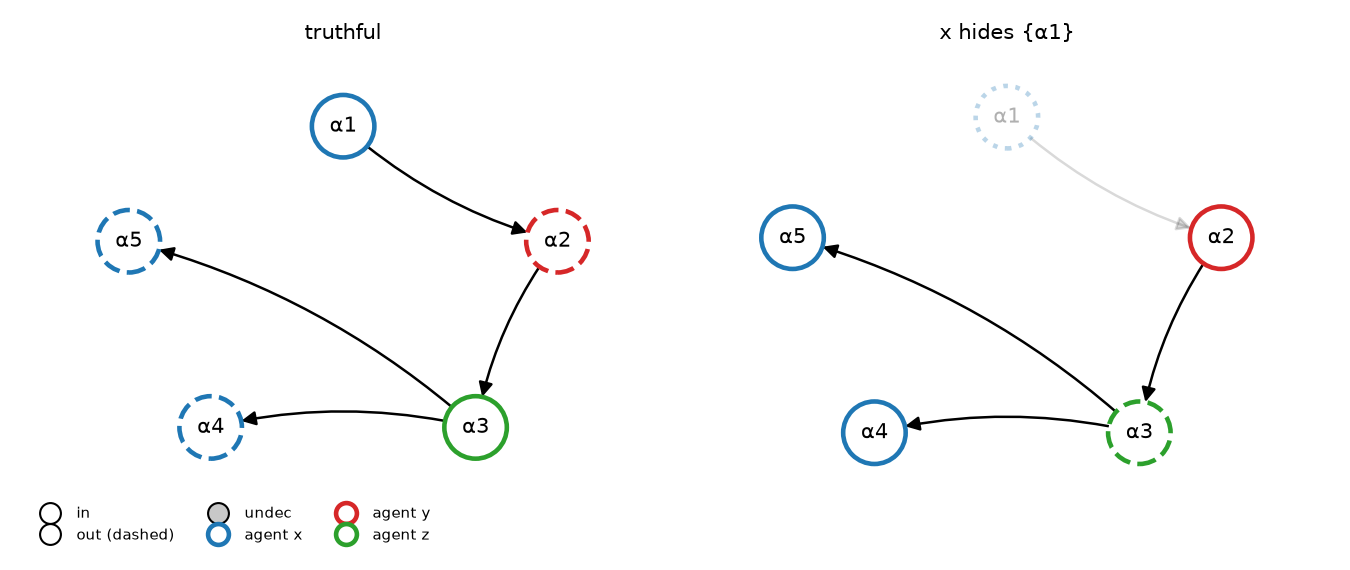
\includegraphics[width=0.66\textwidth]{../demo/figures/example_5_10.png}\\[2pt]
{\sffamily\scriptsize\color{muted}Example 5.10 drawn by the engine. Left: all agents reveal everything, so $x$ gets only $\alpha_1$ accepted.
Right: $x$ hides $\alpha_1$, and $\alpha_4,\alpha_5$ become accepted, so lying pays.}
\end{center}
\vfill
\begin{center}
{\sffamily\small\bfseries\color{brand}Submitted by (group)}\par\smallskip
\begin{tabular}{l l}
{\sffamily\bfseries\color{brand}Nisarg Upadhyay} & {\sffamily\color{muted}B23CS1075}\\[2pt]
{\sffamily\bfseries\color{brand}Mohit Meemrauth} & {\sffamily\color{muted}B23CS1038}\\[2pt]
{\sffamily\bfseries\color{brand}Divyansh Maheshwari} & {\sffamily\color{muted}B23CM1015}\\[2pt]
{\sffamily\bfseries\color{brand}Tejas Kalkar} & {\sffamily\color{muted}B23CM1051}
\end{tabular}

\vspace{0.4cm}
{\sffamily\small\color{muted}November 2026}
\end{center}
\end{titlepage}

% ---------------------------------------------------------------- contents
\pagenumbering{roman}
{\hypersetup{linkcolor=brand}\sffamily
\renewcommand{\contentsname}{\color{brand}Contents}
\tableofcontents}
\markboth{Contents}{}
\clearpage
\pagenumbering{arabic}

% ============================================================================
\section{Introduction}

An \emph{argumentation framework} keeps only which argument attacks which; a \emph{semantics} decides which sets of
arguments can be accepted together (Dung 1995). Chapter~5 of Weiss's \emph{Multiagent Systems} (Rahwan) develops this theory
and then asks a mechanism-design question: if self-interested agents each hold some of the arguments and the outcome is the
grounded extension, can an agent gain by \emph{hiding} arguments?

Part~1 of the assignment builds an argumentation engine; Part~2 implements the grounded direct argumentation mechanism and
studies, on random instances, how often it is strategyproof and how well Theorem~5.4 predicts this.

\begin{keybox}[Headline results]
\begin{itemize}
  \item \textbf{All book examples are reproduced}, and both misprints named in the brief are confirmed: in Example~5.10,
        $u_y$ and $u_z$ are printed with each other's argument sets; after Example~5.11, the argument that cancels $x$'s
        indirect self-defeat is $\alpha_6$, not $\alpha_5$.
  \item \textbf{Q1.} Strategyproof fraction: \textbf{0.628}, \textbf{0.284} and \textbf{0.105} for $p = 0.15, 0.25, 0.35$.
  \item \textbf{Q2. None.} No instance satisfies the Theorem~5.4 condition yet fails strategyproofness, under any reading of
        ``odd-length path''. A further search over \StressGrandTotal{} instances agrees, and we prove why.
  \item \textbf{Q3. Yes, 876 instances} (82--97\,\% of all strategyproof ones), all explained: 856 \emph{offset}, 2
        \emph{self-neutralised} (as in Example~5.11), 18 \emph{dormant}.
\end{itemize}
\end{keybox}

\begin{table}[H]\centering
\caption{Assignment items and where they are met.}\label{tab:req}
\small
\begin{tabularx}{\textwidth}{>{\raggedright\arraybackslash}X >{\raggedright\arraybackslash}p{7.0cm} >{\raggedright\arraybackslash}p{1.3cm} c}
\rowcolor{brand}\thd{Requirement} & \thd{Function} & \thd{Section} & \thd{}\\
\rowcolor{white} 1 Framework class $\AF$ & \code{ArgumentationFramework} (alias \code{AF}) & \S\ref{sec:engine} & \yes\\
\rowcolor{rowalt} 2 Conflict-free test & \code{is\_conflict\_free(af, S)} & \S\ref{sec:engine} & \yes\\
\rowcolor{white} 3 Is $\alpha$ defended by $S$? & \code{defends(af, S, a)} & \S\ref{sec:engine} & \yes\\
\rowcolor{rowalt} 4 Characteristic function & \code{characteristic\_function(af, S)} & \S\ref{sec:engine} & \yes\\
\rowcolor{white} 5 Admissible / complete & \code{is\_admissible}, \code{is\_complete\_extension} & \S\ref{sec:engine} & \yes\\
\rowcolor{rowalt} 6A Grounded extension & \code{grounded\_extension}, \code{grounded\_trace} & \S\ref{sec:semantics} & \yes\\
\rowcolor{white} 6B All complete extensions & \code{complete\_extensions} & \S\ref{sec:semantics} & \yes\\
\rowcolor{rowalt} 6C Preferred, stable, semi-stable & \code{preferred\_/stable\_/semi\_stable\_extensions}, \code{all\_extensions} & \S\ref{sec:semantics} & \yes\\
\rowcolor{white} 6D All legal labellings & \code{all\_labellings}, \code{is\_legal} & \S\ref{sec:semantics} & \yes\\
\rowcolor{rowalt} 6E Acceptance status & \code{acceptance\_status(af, a, semantics)} & \S\ref{sec:semantics} & \yes\\
\rowcolor{white} Test on the book's examples & 161 automated tests & \S\ref{sec:validation} & \yes\\
\rowcolor{rowalt} S1 Mechanism & \code{grounded\_mechanism(R, reports)} & \S\ref{sec:part2} & \yes\\
\rowcolor{white} S2 Best responses & \code{best\_responses(R, types, i, others)} & \S\ref{sec:part2} & \yes\\
\rowcolor{rowalt} S3 Theorem 5.3 check & \code{is\_strategyproof(R, types)} & \S\ref{sec:part2} & \yes\\
\rowcolor{white} S4 Theorem 5.4 condition (with cycles) & \code{theorem\_5\_4\_condition(R, types, mode)} & \S\ref{sec:t54} & \yes\\
\rowcolor{rowalt} Experiments Q1, Q2, Q3 & \code{experiments/run\_experiments.py}, \code{analyse.py} & \S\ref{sec:experiments} & \yes\\
\rowcolor{white} Book misprints & confirmed by the engine and by tests & \S\ref{sec:misprints} & \yes\\
\rowcolor{rowalt} Code, Readme, Report, Demonstration & \code{argengine/}, \code{README.md}, this report, \code{demo/} & \S\ref{sec:demo} & \yes\\
\tabend
\end{tabularx}
\end{table}

% ============================================================================
\section{Background}\label{sec:background}

Definitions follow Weiss (ed.), \emph{Multiagent Systems}, 2nd ed., Ch.~5. In the code, $\alpha_k$ is written \code{"ak"}.

\begin{defbox}{Abstract argumentation (Defs.~5.1--5.8)}
An argumentation framework is $\AF$ with a finite set of arguments $\Args$ and an attack relation ${\att}\subseteq\Args\times\Args$.
Let $\alpha^-$ be the attackers of $\alpha$ and $S^+$ the arguments attacked by $S$.
\begin{itemize}
  \item $S$ is \textbf{conflict-free} iff $S\cap S^+=\emptyset$; $S$ \textbf{defends} $\alpha$ iff $\alpha^-\subseteq S^+$;
        the \textbf{characteristic function} is $F(S)=\{\alpha\mid S \text{ defends } \alpha\}$.
  \item A conflict-free $S$ is \textbf{admissible} iff $S\subseteq F(S)$ and \textbf{complete} iff $S=F(S)$.
  \item \textbf{Grounded}: the least complete extension (least fixed point of $F$). \textbf{Preferred}: maximal complete
        extensions. \textbf{Stable}: $S^+=\Args\setminus S$. \textbf{Semi-stable}: complete extensions with maximal range
        $S\cup S^+$.
  \item A \textbf{legal labelling} $L:\Args\to\{\textsf{in},\textsf{out},\textsf{undec}\}$: $\alpha$ is \textsf{out} iff some
        attacker is \textsf{in}, \textsf{in} iff all attackers are \textsf{out}, otherwise \textsf{undec}. Legal labellings
        correspond one to one to complete extensions ($\textsf{in}=S$, $\textsf{out}=S^+$).
  \item $\alpha$ is \textbf{skeptically accepted} if it is in every extension, \textbf{credulously accepted} if in some, and
        \textbf{rejected} if in none.
\end{itemize}
\end{defbox}

\begin{defbox}{Strategic argumentation (Defs.~5.17--5.22, Theorems 5.3, 5.4)}
Agent $i$ holds a \emph{type} $\Args_i\subseteq\Args$ and reports any subset $\Args^\circ_i\subseteq\Args_i$ (agents lie only by
hiding). The outcome is the grounded extension of the graph induced by $\bigcup_i\Args^\circ_i$, and the utility is
$u_i(o)=|\Args_i\cap o|$. The mechanism is \textbf{strategyproof} iff revealing $\Args_i$ is a best response for every agent
against every combination of the others' reports (the condition checked for Theorem~5.3).
\textbf{Theorem 5.4:} if no agent holds $\alpha,\beta$ with an \emph{odd-length} directed path $\alpha\rightsquigarrow\beta$
(an indirect defeat $\alpha\idef\beta$; length~1 is a direct attack), the mechanism is strategyproof.
\end{defbox}

% ============================================================================
\section{Part 1: the argumentation engine}\label{sec:part1}

\subsection{Framework class and basic tests (items 1--5)}\label{sec:engine}

\code{ArgumentationFramework(arguments, attacks)} stores $\AF$. The API takes and returns ordinary Python sets of names.
Internally, argument $\alpha_i$ is bit $i$ and every set is an integer \emph{bitmask}; for each argument the class
precomputes the masks of its attackers and targets. The basic tests then become a few bit operations:
\begin{itemize}
  \item \code{is\_conflict\_free(af, S)}: $S^+\wedge S=0$, where $S^+$ is the OR of the target masks of $S$;
  \item \code{defends(af, S, a)}: $\texttt{attackers}[\alpha]\wedge\neg S^+=0$;
  \item \code{characteristic\_function(af, S)}: all $\alpha$ with that property, i.e.\ $F(S)$;
  \item \code{is\_admissible}: conflict-free and $S\subseteq F(S)$; \code{is\_complete\_extension}: conflict-free and $S=F(S)$.
\end{itemize}
Because every subset of $\Args$ is an integer in $[0,2^n)$, subsets can be enumerated and results cached cheaply, which
Part~2 relies on. Unknown arguments raise an error, and \code{restrict(S)} returns the induced sub-framework.

\subsection{Semantics, labellings and acceptance (items 6A--6E)}\label{sec:semantics}

\begin{algobox}{Algorithms 1--2 -- grounded and complete extensions}
\begin{algo}
  \item \kw{Grounded:} $S\gets\emptyset$; \kw{repeat} $S\gets F(S)$ \kw{until} $S$ does not change \cmt{at most $n+1$ rounds}
  \item \kw{Complete:} $G\gets$ grounded; $\mathit{free}\gets\Args\setminus(G\cup G^+)$
  \item \ind \kw{for} every $X\subseteq\mathit{free}$: \kw{if} $S=G\cup X$ is conflict-free \kw{and} $F(S)=S$ \kw{then} output $S$
\end{algo}
\end{algobox}

\begin{itemize}
  \item \textbf{6A Grounded.} $F$ is monotone, so iterating it from $\emptyset$ reaches the least fixed point.
        \code{grounded\_trace} returns $F^1(\emptyset), F^2(\emptyset), \dots$ as in the book.
  \item \textbf{6B Complete.} Every complete extension contains the grounded extension $G$ and, being conflict-free, nothing in
        $G^+$; so only subsets of the remaining ``free'' arguments must be tried. This is exact and much smaller than $2^n$.
  \item \textbf{6C Preferred / stable / semi-stable} are selected from the complete extensions: the $\subseteq$-maximal ones; those
        with $S^+=\Args\setminus S$; and those with $\subseteq$-maximal range $S\cup S^+$. \code{all\_extensions} returns all five
        semantics at once.
  \item \textbf{6D Labellings.} Each complete extension $S$ gives the labelling $\textsf{in}=S$, $\textsf{out}=S^+$,
        $\textsf{undec}=$ the rest. \code{is\_legal} checks the definition directly, and a $3^n$ brute force confirms that no
        legal labelling is missed. Table~5.1 is implemented as selectors (min/max \textsf{in}, min/empty \textsf{undec}).
  \item \textbf{6E Acceptance status.} \code{acceptance\_status(af, a, semantics)} returns skeptically accepted, credulously
        accepted or rejected for any of the five semantics; \code{status\_table} lists all arguments.
\end{itemize}

\begin{notebox}[Design decision: no extension]
Under stable semantics an odd cycle has \emph{no} extension, so ``in every extension'' is vacuously true. We report such
arguments as \textbf{rejected} (with \code{n\_extensions = 0}), not as skeptically accepted.
\end{notebox}

% ============================================================================
\section{Validation on the book's examples}\label{sec:validation}

Each row of Table~\ref{tab:book} is an automated test (161 tests in total, \code{pytest}) and is printed by the demonstration.

\begin{table}[H]\centering
\caption{Book statements and engine output (identical).}\label{tab:book}
\small
\begin{tabularx}{\textwidth}{>{\raggedright\arraybackslash}p{2.4cm} X c}
\rowcolor{brand}\thd{Example} & \thd{Book statement = engine output} & \thd{}\\
\rowcolor{white} Fig.~5.1, Ex.~5.5 & $\{\al1,\al3,\al5\}$ conflict-free, $\{\al1,\al2\}$ not; $\emptyset,\{\al3\},\{\al5\},\{\al3,\al5\},\{\al1,\al3,\al5\}$ admissible & \yes\\
\rowcolor{rowalt} Fig.~5.1, Ex.~5.6 & $\{\al3,\al5\}$ defends $\al1$, $\{\al3\}$ does not; $F(\{\al3\})=F(\{\al5\})=\{\al3,\al5\}$; $\{\al3,\al5\}$ admissible but not complete; only complete extension $\{\al1,\al3,\al5\}$ & \yes\\
\rowcolor{white} Fig.~5.1, p.~184 & $F^1(\emptyset)=\{\al3,\al5\}$, $F^2(\emptyset)=F^3(\emptyset)=\{\al1,\al3,\al5\}$ = grounded & \yes\\
\rowcolor{rowalt} Fig.~5.2, Ex.~5.7, 5.8 & complete: $\{\al3\},\{\al1,\al3\},\{\al2,\al3\}$ (three labellings); grounded $\{\al3\}$; preferred $\{\al1,\al3\},\{\al2,\al3\}$; $\al3$ skeptically, $\al1,\al2$ credulously accepted & \yes\\
\rowcolor{white} Fig.~5.3, Ex.~5.9 & grounded $=\{a,c,e\}$ ($F^1=\{e\}$, $F^2=\{c,e\}$, $F^3=\{a,c,e\}$) & \yes\\
\rowcolor{rowalt} Ex.~5.10, 5.11 & see Table~\ref{tab:ex510} & \yes\\
\tabend
\end{tabularx}
\end{table}

\begin{figure}[H]\centering
\begin{subfigure}[b]{0.30\textwidth}\centering
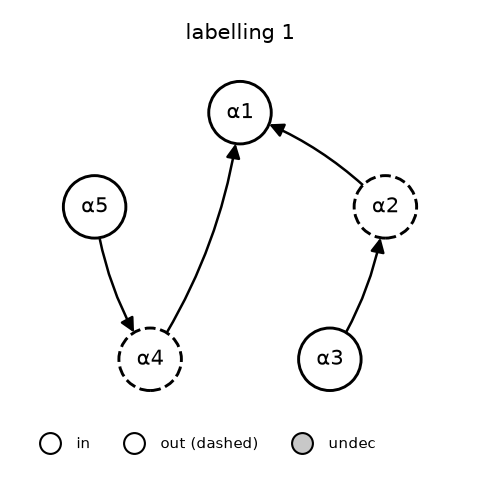
\includegraphics[width=\textwidth]{../demo/figures/figure_5_1.png}
\caption{Fig.~5.1: grounded $\{\al1,\al3,\al5\}$.}
\end{subfigure}\\[4pt]
\begin{subfigure}[b]{0.85\textwidth}\centering
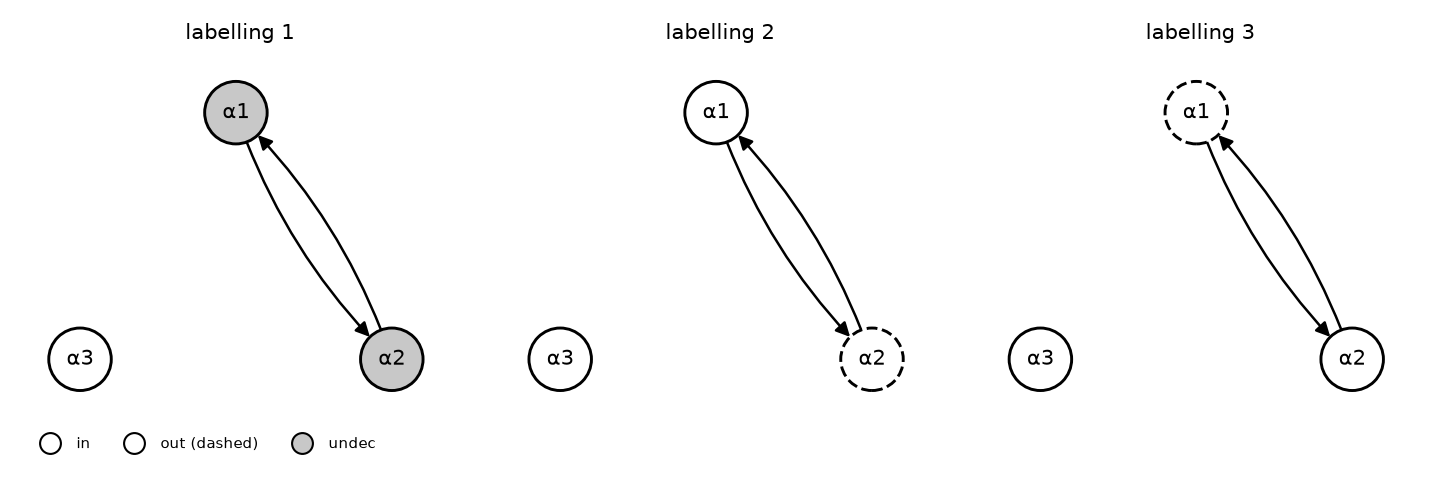
\includegraphics[width=\textwidth]{../demo/figures/figure_5_2.png}
\caption{Fig.~5.2: the three legal labellings.}
\end{subfigure}
\caption{Book frameworks drawn by the engine: solid border = \textsf{in}, dashed = \textsf{out}, grey = \textsf{undec}.}\label{fig:book}
\end{figure}

The book's frameworks do not separate preferred, stable and semi-stable, so we added the frameworks of
Table~\ref{tab:extra}; Table~\ref{tab:acc} shows that the acceptance status changes with the semantics as expected.
Property-based tests (\emph{hypothesis}, hundreds of random frameworks) also check that grounded $\subseteq$ every complete
extension, stable $\subseteq$ semi-stable $\subseteq$ preferred $\subseteq$ complete, preferred = maximal admissible, and that the
labellings agree with the $3^n$ brute force.

\begin{table}[H]\centering
\caption{Extra frameworks (``none'' = no extension exists).}\label{tab:extra}
\small
\begin{tabularx}{\textwidth}{>{\raggedright\arraybackslash}p{3.3cm} >{\raggedright\arraybackslash}p{3.6cm} X X X}
\rowcolor{brand}\thd{Framework} & \thd{Attacks} & \thd{Complete} & \thd{Preferred} & \thd{Stable / semi-stable}\\
\rowcolor{white} Odd 3-cycle & $a\att b\att c\att a$ & $\emptyset$ & $\emptyset$ & none / $\emptyset$\\
\rowcolor{rowalt} Preferred $\ne$ semi-stable & $a\rightleftarrows b$, $b\att c$, $c\att d\att e\att c$ & $\emptyset,\{a\},\{b,d\}$ & $\{a\},\{b,d\}$ & $\{b,d\}$ / $\{b,d\}$\\
\rowcolor{white} Semi-stable without stable & $a\rightleftarrows b$, $b\att c$, $c\att c$, $d\att e\att f\att d$ & $\emptyset,\{a\},\{b\}$ & $\{a\},\{b\}$ & none / $\{b\}$\\
\tabend
\end{tabularx}
\end{table}

\begin{table}[H]\centering
\caption{Item 6E: acceptance status by semantics (S = skeptically, C = credulously accepted, R = rejected).}\label{tab:acc}
\small
\begin{tabular}{l l c c c c c}
\rowcolor{brand}\thd{Framework} & \thd{Argument} & \thd{grounded} & \thd{complete} & \thd{preferred} & \thd{stable} & \thd{semi-stable}\\
\rowcolor{white} Fig.~5.2 & $\al1$, $\al2$ & R & C & C & C & C\\
\rowcolor{white}         & $\al3$ & S & S & S & S & S\\
\rowcolor{rowalt} Pref.\ $\ne$ semi-stable & $a$ & R & C & C & R & R\\
\rowcolor{rowalt}         & $b$, $d$ & R & C & C & S & S\\
\rowcolor{white} Semi-stable w/o stable & $b$ & R & C & C & R (none) & S\\
\tabend
\end{tabular}
\end{table}

% ============================================================================
\section{Part 2: the grounded direct argumentation mechanism}\label{sec:part2}

\subsection{Mechanism, best responses and strategyproofness (items 1--3)}

\begin{itemize}
  \item \textbf{Mechanism.} \code{grounded\_mechanism(R, reports)} builds the graph induced by the union of the revealed sets
        under the global attack relation \code{R} and returns its grounded extension (Part~1 code).
        \code{MechanismInstance} caches the outcome of every revealed set (at most $2^n=256$ for $n=8$), so repeated queries are
        look-ups.
  \item \textbf{Best responses.} \code{best\_responses(R, types, i, others)} enumerates all $2^{|\Args_i|}$ reports of agent $i$
        against the fixed reports of the others and returns \emph{every} utility-maximising report, plus whether truth-telling
        is among them (ties are common).
  \item \textbf{Strategyproofness.} \code{is\_strategyproof(R, types)} runs Algorithm~3 and returns a \emph{witness} (the
        others' reports, what the agent hides, and both utilities) for every manipulable agent.
\end{itemize}

\begin{algobox}{Algorithm 3 -- strategyproofness check (Theorem 5.3 condition)}
\begin{algo}
  \item \kw{for} each agent $i$, \kw{for} every $O\subseteq\bigcup_{j\ne i}\Args_j$ \cmt{every possible union of the others' reports}
  \item \ind $u_T\gets|\Args_i\cap g(\Args_i\cup O)|$ \cmt{truthful utility}
  \item \ind \kw{if} some $S\subseteq\Args_i$ has $|\Args_i\cap g(S\cup O)|>u_T$ \kw{then} record a witness
  \item \kw{return} strategyproof $\iff$ no witness
\end{algo}
\end{algobox}

The outcome depends on the reports only through their union, and the others can produce exactly every subset of the union of
their types, so this covers every combination of the others' reports. A brute-force version that enumerates the profiles
agent by agent agrees with it in the tests.

\subsection{The Theorem 5.4 condition on cyclic graphs (item 4)}\label{sec:t54}

\code{theorem\_5\_4\_condition} checks the \emph{full} graph for two arguments of the same agent joined by an odd-length
path, and returns each violating path. On a cyclic graph, ``odd-length path'' has two readings, and a naive path search may
loop forever; both readings are implemented safely:
\begin{itemize}
  \item \textbf{Odd simple path} (no repeated vertex; default, the literal graph-theory meaning): DFS with a visited set, so it
        always terminates; exact for $n\le8$.
  \item \textbf{Odd walk} (vertices may repeat): BFS over states (vertex, parity of the length). Each state is visited once,
        so cycles cannot cause non-termination; an odd cycle just makes a vertex reachable with both parities.
\end{itemize}
A flag \code{include\_self} decides whether $\alpha=\beta$ (a self-attack or an odd cycle through one owned argument) counts.
The experiments report all four combinations.

\subsection{Examples 5.10 and 5.11}\label{sec:ex510}

\begin{table}[H]\centering
\caption{Examples 5.10 and 5.11. Types $x=\{\al1,\al4,\al5\}$ (+$\al6$ in 5.11), $y=\{\al2\}$, $z=\{\al3\}$; attacks
$\al1\att\al2\att\al3$, $\al3\att\al4$, $\al3\att\al5$ (+$\al6\att\al3$ in 5.11).}\label{tab:ex510}
\small
\begin{tabularx}{\textwidth}{>{\raggedright\arraybackslash}p{4.0cm} X X}
\rowcolor{brand}\thd{} & \thd{Example 5.10} & \thd{Example 5.11}\\
\rowcolor{white} Truthful outcome & $\{\al1,\al3\}$ & $\{\al1,\al4,\al5,\al6\}$\\
\rowcolor{rowalt} Utilities $u_x,u_y,u_z$ & $1,\ 0,\ 1$ & $4,\ 0,\ 0$\\
\rowcolor{white} $x$'s best response & $\{\al4,\al5\}$ (\textbf{hide $\al1$}), utility 2 & reveal everything, utility 4 (hiding $\al1$ gives $\{\al2,\al4,\al5,\al6\}$, utility 3)\\
\rowcolor{rowalt} Strategyproof? & \no\ ($x$ hides $\al1$: outcome $\{\al2,\al4,\al5\}$) & \yes\\
\rowcolor{white} Thm 5.4 condition & fails: $\al1\att\al2\att\al3\att\al4$ (and $\al5$) & fails: same paths\\
\tabend
\end{tabularx}
\end{table}

In Example~5.10, $\al1$ defeats $\al2$, which reinstates $\al3$, which defeats $x$'s own $\al4$ and $\al5$; hiding $\al1$ loses one
accepted argument and gains two (title-page figure). In Example~5.11, $\al6$ defeats $\al3$ whatever happens to $\al1$, so hiding
no longer helps: the mechanism is strategyproof even though the condition fails, the first example of Q3.

\begin{notebox}[Misprints in the book (confirmed)]\label{sec:misprints}
\begin{itemize}
  \item \textbf{Example 5.10:} the book prints $u_y(o,\{\al3\})=1$ and $u_z(o,\{\al2\})=0$; the correct values are
        $u_y(o,\{\al2\})=0$ and $u_z(o,\{\al3\})=1$ for $o=\{\al1,\al3\}$.
  \item \textbf{After Example 5.11:} the argument that cancels $x$'s indirect self-defeat is $\al6$, not $\al5$. With $\al6$ in
        $x$'s type the mechanism is strategyproof; without it, it is not. $\al5$ attacks nothing, so it cannot cancel anything.
\end{itemize}
\end{notebox}

% ============================================================================
\section{Experiments}\label{sec:experiments}

\textbf{Setup.} 3 agents; $n\sim U\{6,7,8\}$ arguments; each ordered pair $(\alpha,\beta)$, $\alpha\ne\beta$, is an attack with
probability $p\in\{0.15,0.25,0.35\}$; each argument is given to one agent uniformly at random (types are disjoint and may be
empty); \textbf{1000 instances per $p$}, seed 2026. For each instance we record whether the mechanism is strategyproof
(Algorithm~3) and whether the Theorem~5.4 condition holds under each reading. Results are exact; the whole run takes about
3~s. Raw data: \code{experiments/results/instances.csv}.

\subsection{Q1: fraction of strategyproof instances}\label{sec:q1}

\begin{table}[H]\centering
\caption{Q1 -- strategyproofness by attack probability (95\,\% Wilson intervals).}\label{tab:q1}
\small
\begin{tabular}{c c c c c c c c}
\rowcolor{brand}\thd{$p$} & \thd{SP} & \thd{fraction} & \thd{95\,\% CI} & \thd{$n=6\,/\,7\,/\,8$} & \thd{acyclic} & \thd{cyclic} & \thd{Thm 5.4 holds}\\
\rowcolor{white} 0.15 & 628 & \textbf{0.628} & [0.598, 0.657] & 0.74 / 0.62 / 0.52 & 0.89 & 0.34 & 0.111\\
\rowcolor{rowalt} 0.25 & 284 & \textbf{0.284} & [0.257, 0.313] & 0.43 / 0.28 / 0.14 & 0.87 & 0.18 & 0.027\\
\rowcolor{white} 0.35 & 105 & \textbf{0.105} & [0.087, 0.126] & 0.22 / 0.08 / 0.03 & 0.89 & 0.08 & 0.003\\
\tabend
\end{tabular}
\end{table}

\begin{figure}[tbp]\centering
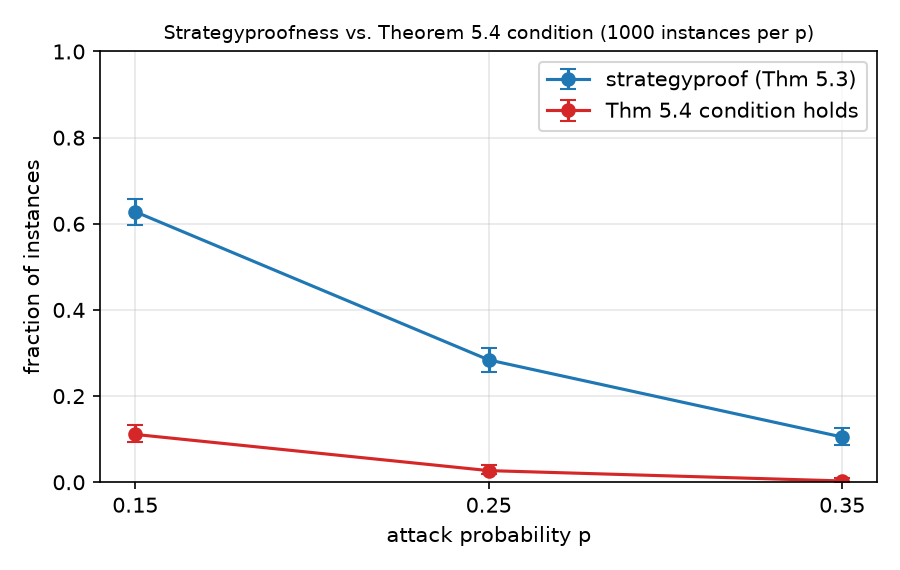
\includegraphics[width=0.62\textwidth]{../experiments/results/fig_sp_vs_p.png}
\caption{Q1: fraction of strategyproof instances and of instances satisfying the Theorem~5.4 condition.}\label{fig:q1}
\end{figure}

\begin{keybox}[Q1 -- findings]
\begin{itemize}
  \item Strategyproofness becomes rare as the graph gets denser (63\,\% $\to$ 28\,\% $\to$ 11\,\%) and as $n$ grows: more
        attacks create more odd paths between arguments of the same agent, and such a path is needed to gain by hiding.
  \item Cycles drive the effect: acyclic instances are strategyproof 87--89\,\% of the time at every $p$, cyclic ones only
        8--34\,\%; the share of cyclic graphs grows from 47\,\% to 97\,\%.
  \item The Theorem~5.4 condition holds far less often than strategyproofness (11.1\,\%, 2.7\,\%, 0.3\,\%).
\end{itemize}
\end{keybox}

\subsection{Q2: condition holds but not strategyproof -- none}\label{sec:q2}

\begin{table}[H]\centering
\caption{Theorem 5.4 condition $\times$ strategyproofness, for $p = 0.15\,/\,0.25\,/\,0.35$. Q2 = condition holds $\wedge$ not SP.}\label{tab:q2}
\small
\begin{tabularx}{\textwidth}{>{\raggedright\arraybackslash}X c c c c}
\rowcolor{brand}\thd{Reading of ``odd-length path''} & \thd{cond $\wedge$ SP} & \thd{\textbf{Q2}} & \thd{Q3: $\neg$cond $\wedge$ SP} & \thd{$\neg$cond $\wedge\neg$SP}\\
\rowcolor{ennbg} simple path, $\alpha=\beta$ allowed (\textbf{primary}) & 111 / 27 / 3 & \textbf{0 / 0 / 0} & 517 / 257 / 102 & 372 / 716 / 895\\
\rowcolor{white} walk, $\alpha=\beta$ allowed & 111 / 27 / 3 & \textbf{0 / 0 / 0} & 517 / 257 / 102 & 372 / 716 / 895\\
\rowcolor{rowalt} simple path, $\alpha\ne\beta$ & 113 / 29 / 3 & \textbf{0 / 0 / 0} & 515 / 255 / 102 & 372 / 716 / 895\\
\rowcolor{white} walk, $\alpha\ne\beta$ & 112 / 27 / 3 & \textbf{0 / 0 / 0} & 516 / 257 / 102 & 372 / 716 / 895\\
\tabend
\end{tabularx}
\end{table}

No instance satisfies the condition yet fails strategyproofness, under any reading. To rule out luck,
\code{experiments/stress\_test.py} also checked \emph{every} 3-agent instance with $n\le\StressMaxN$ arguments
(\StressExTotal{} instances, self-attacks allowed) and \StressRandTotal{} further random ones, using the weakest reading: again
\textbf{0} counterexamples. This is expected, because Theorem~5.4 holds on cyclic graphs, even in a sharper form:

\begin{defbox}{Lemma and sharpened Theorem 5.4}
\textbf{Lemma.} If hiding $S$ from the revealed set $M$ turns an argument $\beta$ \textsf{in}
($\beta\in\GE(M\setminus S)\setminus\GE(M)$), then some $\alpha\in S$ has an odd \emph{simple} path $\alpha\rightsquigarrow\beta$ in the
graph induced by $M$.\\[2pt]
\textbf{Theorem.} If no agent holds two \emph{distinct} arguments joined by an odd simple path in the full graph, the
mechanism is strategyproof.
\end{defbox}

\textbf{Proof sketch.} $\beta\notin\GE(M)$, so some attacker $\gamma$ of $\beta$ is not defeated by $\GE(M)$. If $\gamma\in S$, the path
$\gamma\att\beta$ has length~1. Otherwise $\gamma$ is defeated in $\GE(M\setminus S)$ by some $\delta$ that is itself newly \textsf{in}, at
an earlier stage of the fixed-point iteration; by induction an odd path leads from $S$ to $\delta$, and $\delta\att\gamma\att\beta$ adds two
edges, keeping it odd. Repeated vertices can only be $\gamma$'s, and removing the loop between them removes an even number of edges,
so the path can be made simple. For the theorem: a gaining agent has some own $\beta$ newly \textsf{in}, so the lemma gives an odd
path from one of its own hidden $\alpha\ne\beta$ to $\beta$, a contradiction.~\qedbox

All four readings in Table~\ref{tab:q2} forbid at least as much as this one, so \textbf{Q2 must be empty}. The lemma was also
confirmed on the witness of all 1983 manipulable instances.

\subsection{Q3: strategyproof although the condition fails}\label{sec:q3}

\begin{table}[H]\centering
\caption{Q3 -- strategyproof instances that violate the (primary) Theorem 5.4 condition, by explanation.}\label{tab:q3}
\small
\begin{tabular}{c c c c c c}
\rowcolor{brand}\thd{$p$} & \thd{SP but cond.\ fails} & \thd{share of all SP} & \thd{offset} & \thd{self-neutralised} & \thd{dormant}\\
\rowcolor{white} 0.15 & 517 & 0.823 & 506 & 2 & 9\\
\rowcolor{rowalt} 0.25 & 257 & 0.905 & 249 & 0 & 8\\
\rowcolor{white} 0.35 & 102 & 0.971 & 101 & 0 & 1\\
\rowcolor{ennbg} \textbf{total} & \textbf{876} & & \textbf{856} & \textbf{2} & \textbf{18}\\
\tabend
\end{tabular}
\end{table}

Yes, and they are the norm: 876 of the 1{,}017 strategyproof instances (86\,\%) violate the condition. Theorem~5.4 only asks whether an odd path \emph{exists}; it ignores whether hiding actually makes
the target \textsf{in}, and whether the gain outweighs the loss. \code{classify\_agent} checks every revealed set and every hidden
set and puts each violating agent in one of three classes:

\begin{itemize}
  \item \textbf{Offset (856).} Hiding does free one of the agent's arguments, but the agent always loses at least as many,
        usually the hidden argument itself, so the net gain is $\le0$ (per agent: 1048 of 1195 are exact swaps with net change 0,
        147 always lose strictly). In 472 of these instances the only violation is a direct
        attack inside a type: in \#224, $y$ owns $\al1\att\al4$ and can trade $\al1$ for $\al4$ but never gain. In \#254,
        $x=\{\al2,\al4\}$ with $\al2\att\al6\att\al1\att\al4$: hiding $\al2$ frees $\al4$ but loses $\al2$. Example~5.10 is the case
        where the trade is \emph{not} balanced (hiding one argument frees two).
  \item \textbf{Self-neutralised (2).} The Example~5.11 pattern: hiding helps only if the agent also withholds another of its
        own arguments, which otherwise blocks the gain. In \#296, $z=\{\al1,\al2,\al4\}$ has $\al4\att\al5\att\al6\att\al1$; hiding
        $\al4$ would free $\al1$ only while $z$ withholds $\al2$, since $\al2\att\al6$ keeps $\al6$ \textsf{out} anyway (Figure~\ref{fig:q3}).
  \item \textbf{Dormant (18).} The odd path never changes acceptance: (i) an odd cycle through a single owned argument
        ($\alpha=\beta$; hiding it removes the argument itself, \#203); (ii) the path runs into an odd cycle that keeps the target
        \textsf{undec} (\#970); (iii) hiding only turns the target from \textsf{out} into \textsf{undec}, which gives no utility (\#900).
\end{itemize}

\begin{figure}[H]\centering
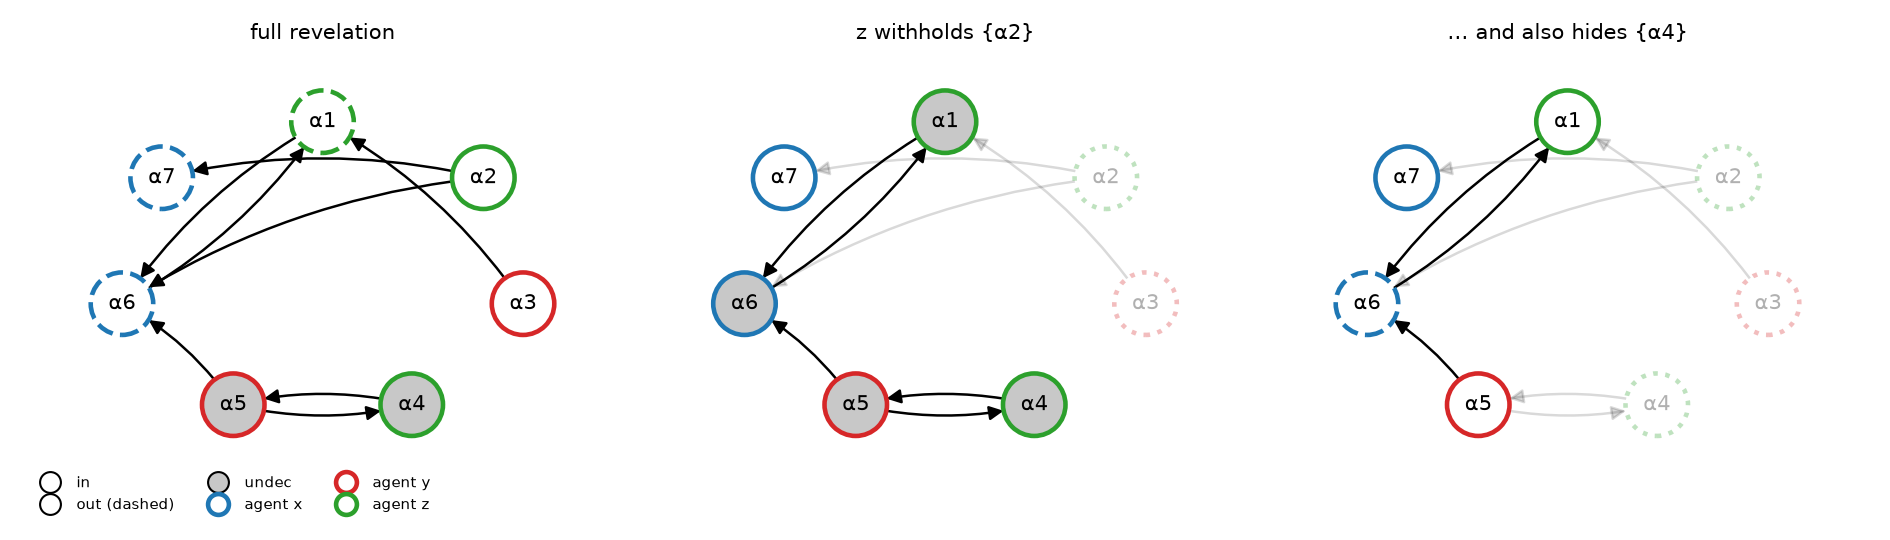
\includegraphics[width=\textwidth]{../experiments/results/examples/q3_self-neutralised_296.png}
\caption{Instance \#296 (self-neutralised). Left: full revelation. Middle: $z$ withholds $\al2$. Right: only then does hiding
$\al4$ turn $\al1$ \textsf{in}. With $\al2$ revealed, $\al6$ is always \textsf{out}, so hiding $\al4$ is useless. Border colour =
owner.}\label{fig:q3}
\end{figure}

\begin{keybox}[Q2 / Q3 -- findings]
\begin{itemize}
  \item Theorem~5.4 is \textbf{sound} (no Q2 instance, and a proof) but \textbf{very conservative}: 82--97\,\% of the
        strategyproof instances violate it.
  \item Nearly all of these (856 of 876) are \emph{offset}: a gain exists but costs as much as it gives. The exact
        Theorem~5.3 check, not the graph condition, characterises strategyproofness.
\end{itemize}
\end{keybox}

% ============================================================================
\section{Demonstration}\label{sec:demo}

\begin{codebox}
python -m pytest -q \hfill{\rmfamily\color{muted}\itshape 161 tests}\\
python -m argengine.demo --part 1 \hfill{\rmfamily\color{muted}\itshape items 1--6E on all book examples}\\
python -m argengine.demo --part 2 \hfill{\rmfamily\color{muted}\itshape Examples 5.10, 5.11 and the misprints}\\
python -m argengine.demo --file demo/inputs/custom\_strategic.json \hfill{\rmfamily\color{muted}\itshape any framework (JSON / .apx)}\\
python experiments/run\_experiments.py \&\& python experiments/analyse.py \hfill{\rmfamily\color{muted}\itshape Q1--Q3}
\end{codebox}

The CLI walks through every item: the basic tests on Figure~5.1, the grounded trace, all extensions, labellings and an
acceptance-status table for every framework; then utilities, best responses, the strategyproofness verdict with a witness
and the Theorem~5.4 violations for Examples~5.10 and 5.11. \code{demo/demo.ipynb} (executed, with drawings) and
\code{demo/demo.html} show the same in notebook form. Setup and all commands are in \code{README.md}.

% ============================================================================
\section{Conclusion}

\code{argengine} implements every function asked for in Part~1 and reproduces all examples of Chapter~5. The grounded direct
mechanism has exact best responses, an exact strategyproofness check with witnesses, and the Theorem~5.4 condition under both
readings of ``odd-length path'', safe on cycles. Strategyproofness is common for sparse attack graphs (63\,\% at $p=0.15$) and
rare for dense ones (11\,\% at $p=0.35$). Theorem~5.4 is never wrong but is very conservative; every strategyproof instance that
violates it is explained by an offset, self-neutralising or dormant mechanism. \textbf{Limitations:} enumeration is exponential
in $n$ (fine for $n\le8$; larger frameworks would need SAT/ASP solvers), and agents can only hide arguments, as in the book.

\section*{References}
\addcontentsline{toc}{section}{References}
\begin{enumerate}[label={[\arabic*]},leftmargin=2.2em,itemsep=2pt]
  \item G.~Weiss (ed.), \emph{Multiagent Systems}, 2nd ed., MIT Press, 2013 -- Ch.~5, I.~Rahwan, ``Argumentation among Agents''.
  \item P.~M.~Dung, ``On the acceptability of arguments and its fundamental role in nonmonotonic reasoning, logic programming
        and $n$-person games'', \emph{Artificial Intelligence} 77(2), 1995.
  \item M.~Caminada, ``Semi-stable semantics'', \emph{Proc.\ COMMA}, 2006.
  \item I.~Rahwan, K.~Larson, F.~Tohm\'e, ``A characterisation of strategy-proofness for grounded argumentation semantics'',
        \emph{Proc.\ IJCAI}, 2009.
\end{enumerate}

\end{document}
